\chapter{Estado del Arte}

En los últimos años, el uso de sistemas de localización en interiores ha tomado mucha importancia en una gran cantidad de aplicaciones y contextos. En exteriores, la tecnología de facto es GPS, que sin embargo no presenta buenos resultados en interiores debido a la pobre o nula señal que es recibida en recintos cerrados o bajo tierra. A pesar de que la necesidad de posicionar o monitorear personas u objetos en interiores es alta, los avances no han sido significativos en este campo, debido a la gran cantidad de dificultades que se presentan al momento de resolver este problema como son por ejemplo propagación por múltiples caminos o \textit{Non Line of Sight} (NLoS), es decir, sin línea de visión a los diferentes emisores de señales debido a las condiciones del sistema. También se presentan otros problemas por las condiciones cambiantes del ambiente, por ejemplo, múltiples dispositivos funcionando simultáneamente, alto tránsito de personas y objetos, lo cual atenúa en gran medida las señales o la dispersión de la radiación que es un fenómeno físico frecuente en las ondas de radio.

Claramente no existe una única solución que se adapte a todos los lugares o recintos, ya que cada uno de estos tiene características únicas o en ocasiones se requiere satisfacer ciertos parámetros como por ejemplo costos, exactitud, precisión, escalabilidad, entre otros. Por lo general no es posible optimizar simultáneamente todos estos parámetros nombrados anteriormente, por lo que habitualmente se evalúan las mejores combinaciones de ellos para obtener el mejor desempeño, adaptados a una solución personalizada dependiendo del ambiente en el cual se implementa el sistema de posicionamiento.

\section{Tecnologías para posicionamiento \textit{indoor}}

Una gran cantidad de tecnologías han sido dispuestas para el desarrollo de soluciones al problema de posicionamiento en interiores. Las siguientes secciones muestran las más utilizadas y que a lo largo de múltiples estudios han presentado los mejores resultados.

\subsection{Basado en Visión}

Esta aproximación está basada en el uso de datos provistos mediante cámaras, en formato de vídeo o fotografías. Habitualmente se utilizan dos técnicas para su implementación:

\textbf{Sistemas de cámara fijos:} En este caso el ambiente es equipado con cámaras en diferentes puntos, procurando cubrir la totalidad del recinto. El objetivo entonces consiste en encontrar un objeto en movimiento capturado por una o diversas cámaras. Las características del objeto a rastrear deben ser diferenciadas, con lo cual, cuando estas características sobresalientes están presentes en alguna de las cámaras, es posible obtener la distancia relativa, y por ende, al estar fijas las cámaras, la posición también es obtenida basado en la distribución espacial dentro de las imágenes capturadas.

\textbf{Sistemas de cámaras en movimiento:} El objetivo móvil está equipado con una cámara y la localización se realiza colocando varios puntos de referencia en posiciones conocidas (y orientaciones) o extrayendo características del entorno. Si la cámara móvil detecta dos o más puntos de referencia, puede descubrir su propia posición y orientación. Para ello, el proceso de localización implica dos etapas. En la etapa fuera de línea, imágenes del ambiente se capturan en ubicaciones predefinidas y cada imagen se procesa para extraer sus características únicas para almacenarlas en una base de datos. En la etapa en línea, la cámara captura una imagen y se extraen sus características y se comparan con las características almacenadas para estimar la ubicación de la cámara.

Estas técnicas han alcanzado altos niveles de precisión, inferiores incluso a \(10^{-6} [m]\) para sistemas de alta precisión \citep{6071925}. Por otra parte, la capacidad computacional de vídeo y las altas tasas de procesamiento de datos, sumado a los nuevos algoritmos de compresión y procesamiento de imágenes, hacen de esta tecnología una de las más prometedoras. Un punto desfavorable son sus altos costos, y poca escalabilidad, sin embargo, nuevas formas de utilizar las cámaras de dispositivos móviles están siendo investigadas para desarrollar soluciones de bajo costo manteniendo la eficiencia.

Uno de los acercamientos más osados en el posicionamiento en interiores, es la localización mediante información visual, es decir, basado en imágenes relativas al lugar de exploración. Para el desarrollo de estos modelos habitualmente se usa equipos de vuelo muy pequeños y livianos, los cuales recorren la zona tomando fotografías con el objetivo de \textit{mapear} el recinto.  En \citep{4058367}, los autores utilizan robots de aproximadamente 10 gramos y con una velocidad de vuelo de 1.5 m/s. Estos robots tienen todo lo necesario para regular su velocidad y prevenir colisiones. Estos micro robots están equipados con giroscopios y dos pequeñas cámaras, un pequeño radio control y un módulo Bluetooth. La \autoref{fig:10gr} muestra como están constituidos estos pequeños dispositivos voladores.\\

\begin{figure}[ht!]
\centering
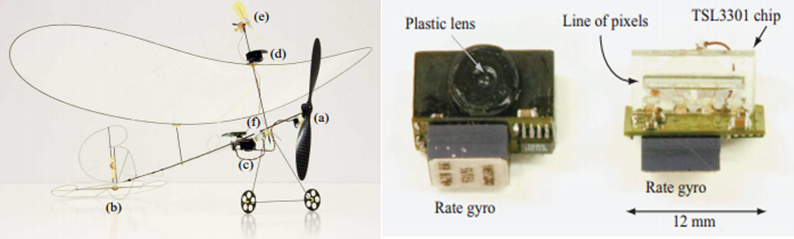
\includegraphics[width=.6\textwidth]{figures/10gr.png}
\caption[Dispositivo volador 10 gramos]{Dispositivo volador que toma imágenes de las murallas para detectar los patrones de textura\\
{\scriptsize (Fuente: \citep{4058367})}}
\label{fig:10gr}
\end{figure}

Estos dispositivos capaces de sobrevolar un recinto pequeño o casas determinan según las texturas de las paredes y su distorsión, la posición relativa dentro del recinto con respecto a la pared fotografiada y utilizando el giroscopio, previenen choques. En la  \autoref{fig:murallas} se observa cómo se generan los patrones de texturas en las murallas para realizar las pruebas.\\

\begin{figure}[ht!]
\centering
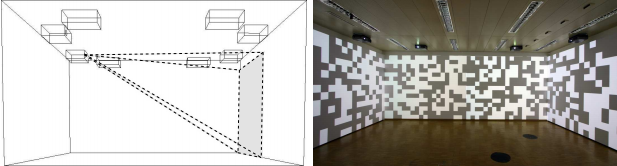
\includegraphics[width=.6\textwidth]{figures/Murallas.png}
\caption[Proyección en murallas vision based]{Proyectores que generan los patrones en las murallas con los cuales los autores realizaron las pruebas\\
{\scriptsize (Fuente: \citep{4058367})}}
\label{fig:murallas}
\end{figure}

Los resultados muestran que la solución es factible, sin embargo no puede controlarse la altitud, y para ello los autores plantean el desarrollo de un \textit{3D visión based tracking system}.

\subsection{Infrarrojo}

La tecnología Infrarroja es una de las más utilizadas para localizar personas y objetos mediante el uso de emisores y receptores infrarrojos.

Una forma posible de utilizar la radiación infrarroja en sistemas de posicionamiento \textit{indoor} es poner en el objeto o persona a localizar, un transmisor infrarrojo con un identificador único. Luego, los receptores son colocados en lugares dentro del recinto, los cuales pueden detectar este identificador único y comunicar a un software especializado, el cual se encarga de calcular la posición mediante la distancia entre el transmisor y receptor. Esta tecnología inalámbrica presenta grandes ventajas. En primer lugar, al no poder atravesar paredes, es fácil confinar las ondas en un recinto. Por otra parte, la radiación infrarroja no se ve afectada por la interferencia electromagnética. A pesar de lo anterior, la tecnología infrarroja presenta dos puntos que lo tornan una opción menos factible. Primero, se ve muy afectado por el efecto de \textit{multipath-propagation}. Además, su implementación requiere hardware y software costoso, por lo que no es tan accesible.

\subsection{Técnicas basadas en Sonido}

La tecnología de ultrasonido utiliza las ondas de ultrasonido para medir la distancia entre una estación base que se encuentra fija, y el objeto a localizar. Para implementar este tipo de sistema, múltiples receptores deben estar sincronizados. Esta sincronización se logra mediante el uso de ondas de radio o radiación infrarroja, ya que estas son mucho más rápidas que las de ultrasonido. El funcionamiento consiste en que los transmisores envían ondas de radio y de ultrasonido al mismo tiempo. Las ondas de radio alcanzan casi instantáneamente a los receptores, con lo cual se pueden sincronizar. Posteriormente cada receptor detecta las ondas de ultrasonido al momento en que arriban, y con esta diferencia de tiempo, es posible calcular la distancia a cada receptor, así se genera una posición relativa dentro de la sala de medición.

Las ventajas de este sistema son los bajos costos de implementación, y la capacidad de funcionar a pesar de la mayoría de las obstrucciones presentes. Las desventajas por su parte son la alta complejidad de desarrollar esta tecnología en sistemas de gran escala, por la sincronización de los receptores. Además la temperatura es uno de los factores más críticos en la velocidad del sonido, es por ello que la gran mayoría de los sistemas basados en ultrasonidos incluyen sensores para compensar estas fluctuaciones de temperatura. Otros factores menos influyentes incluyen la presión del aire, su contenido de dióxido de carbono y la amplitud del sonido.

Otra forma de utilizar el espectro de sonido, y el ultrasonido, es lo que se denomina \textit{acoustic background spectrum}.

En este caso, los autores sugieren una metodología la cual no requiere infraestructura \cite{Tarzia:2011:ILW:1999995.2000011}, es decir las redes inalámbricas son prescindibles. El método consiste en un mapeo \textit{fingerprint} o huella, la cual registra el sonido ambiente de un determinado lugar, y luego construye una base de datos de todas las mediciones realizadas. Posteriormente para estimar la posición del usuario, realiza una comparativa con su actual \textit{fingerprint} y lo contrasta con la base de datos, eligiendo de esta manera la posición más “cercana” según el algoritmo de estimación seleccionado.

El objetivo principal es determinar la posición mediante un dispositivo móvil, como puede ser un Smartphone, de manera rápida y económica a una resolución de una sala de mediano tamaño. La principal ventaja es que no se requiere prácticamente infraestructura por detrás, solo basta los sensores de sonido del equipo móvil.

El principal problema a resolver es entonces traducir los fingerprint a \textit{roomlabels}, es decir la medición actual registrada por el dispositivo móvil, mapearla a una etiqueta de la posición dentro de la sala. Para la realización del fingerprint los autores determinan que este debe ser:

\begin{itemize}
\item Distintivo
\item Responsivo
\item Compacto
\item Eficientemente computable
\item Robusto al ruido
\item Invariante al tiempo
\end{itemize}

Para ello crean \textit{Acoustic background Spectrum} (ABS) que cumple estas condiciones ya que tiene en cuenta ruidos típicos de la vida cotidiana como puede ser sonidos de computadoras, aire acondicionado, entre otros. Para la obtención del \textit{fingerprint} elaboran diversas técnicas basada en el estudio de los sonidos como se aprecia en la  \autoref{fig:abs}.

\begin{figure}[ht!]
\centering
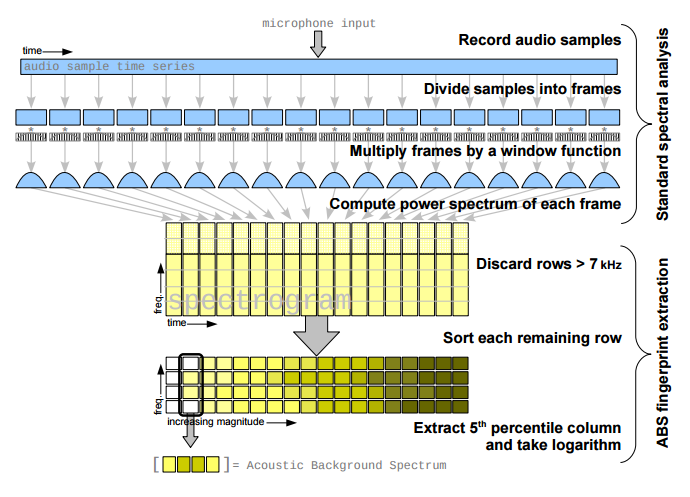
\includegraphics[width=.6\textwidth]{figures/abs.png}
\caption[Método \textit{Acoustic Background Spectrum}]{Descripción del método ABS con el cual se realiza la obtención del mapeo \textit{fingerprint}\\
{\scriptsize (Fuente: \cite{Tarzia:2011:ILW:1999995.2000011})}}
\label{fig:abs}
\end{figure}

Luego de obtener el \textit{fingerprint} los autores usan algoritmos de clasificación, es decir aprendizaje supervisado, como es nearest-neighbor. Se realizaron pruebas en 33 habitaciones distintas, obteniendo una exactitud de 69\%, lo cual muestra resultados aceptables para el posicionamiento utilizando sonidos. Finalmente concluyen que dos \textit{fingerprint} menos exactos pueden ser mejorados si se usan en conjunto, como es el caso de ABS con WiFi.

\subsection{\textit{Wi-Fi}}

\textit{Wireless Local Area Network} (WLAN) puede usarse para estimar la ubicación de un dispositivo móvil dentro de un recinto, dado que la infraestructura WLAN está muy extendida de acuerdo con el aumento de la demanda de redes de comunicaciones, por lo que este enfoque es ampliamente utilizado para posicionamiento \textit{indoor}. Por esta razón, una de las principales ventajas del uso de la técnica de localización Wi-Fi es su rentabilidad ya que no se requiere adicionar infraestructura en lugares donde ya se encuentran estas redes. Otra ventaja de usar WLAN es que no se requiere una línea de visión con los emisores de señales. Es el método más popular que utiliza  \textit{Received Signal Strength Indicator} (RSSI), o intensidad de la señal recibida dentro de las tecnologías inalámbricas y que en este caso son extraídas de las redes IEEE 802.11

En una WLAN, un nodo emite / recibe señales de radiofrecuencia hacia / desde el enrutador inalámbrico, que se puede usar para determinar ubicación precisa de cualquier dispositivo con Wi-Fi habilitado utilizando técnicas que son detalladas posteriormente en esta memoria.

Es la tecnología inalámbrica más utilizada en el mundo, además por seguir un estándar, está claramente definida y sus protocolos funcionan en cualquier parte del mundo. Sus frecuencias son 2.4 GHz y 5 GHz, además es muy escalable utilizando access point, y está muy masificado en dispositivos móviles. Por lo anterior, Wi-Fi se ha vuelto la alternativa más utilizada en técnicas de posicionamiento en interiores.

Recientes investigaciones demuestran que es posible alcanzar una precisión de aproximadamente 3-5 metros \citep{6834746}. Uno de los problemas más grandes son la necesidad de cablear la infraestructura para los routers y el alto consumo de energía que se presenta en ellos. Otro problema presente en la mayoría de las tecnologías inalámbricas es la atenuación de la señal por murallas, objetos o el mismo cuerpo humano.

\subsection{\textit{RFID}}

La tecnología RFID se basa en lectores RFID con una o más antenas, y tags activos o pasivos. Los tags activos poseen una batería, con lo cual son capaces de emitir señales autónomamente, mientras los tag pasivos no poseen batería y requieren de incentivos externos para emitir sus señales. Típicamente se puede poner datos dentro de cada tag, los cuales ayudan a determinar las posiciones. Los datos almacenados dependen estrictamente de la memoria de los tags respectivos.

La localización mediante RFID puede categorizarse en dos tipos, los cuales son localización del lector y localización de tags. En la localización del lector RFID, su precisión depende estrictamente de la densidad de tags dispuestos en el recinto, es decir, la cantidad sobre el área cubierta. Este método funciona de la siguiente manera, el usuario porta un lector y lee los tags dispuestos en distintas posiciones. Cada tag posee información de la posición relativa, con lo cual es fácil reconocer la posición del usuario. Una desventaja obvia, es la poca escalabilidad debido al gran número de tags RFID. 

El segundo método, consiste en determinar la localización del tag RFID. En este caso el usuario no porta un lector, sino que un tag, y los lectores son puestos en lugares estratégicos dentro del recinto, así cuando el usuario transita, los lectores son capaces de determinar en qué lugar fue leído el tag asociado al usuario y determinar su posición. Este método es incluso más costoso que el anterior, ya que los lectores RFID son más caros que los tags. 

Las restricciones más grandes de la tecnología RFID son el corto alcance que este presenta y la posibilidad de leer solo unos pocos tags a la vez. Sin embargo, sus ventajas son muchas, entre ellas se encuentran la alta seguridad de transmisión, alta tasa de transferencia, no requiere línea de visión directa y presenta relativamente bajos costos. 

\subsection{\textit{Bluetooth}}

Bluetooth se ha convertido en el estándar para redes inalámbricas de área personal, WPAN por sus siglas en ingles. Opera en la banda de 2.4 GHz, sin embargo, posee menor alcance que otras tecnologías de radio frecuencia como por ejemplo WLAN, aun a pesar de ello se han registrado implementaciones a gran escala de posicionamiento \textit{indoor} utilizando esta tecnología \citep{BT}. Su rango típicamente alcanza entre 10 a 15 metros, ya que es pensado principalmente para comunicaciones directas entre emisor y receptor dentro de un rango corto, como puede ser una casa o una sala de mediano tamaño. A pesar de esto, el creciente interés de múltiples aplicaciones ha vuelto a la tecnología Bluetooth muy relevante, ya que hoy en día está presente en smartphones, computadores, notebooks entre otros. Con esto presente, no se requiere adicionar mayor hardware a los teléfonos celulares para implementar un sistema de localización, ya que prácticamente todos estos dispositivos cuentan con la tecnología Bluetooth integrada.

Bluetooth es una tecnología de bajo consumo energético y bajo costo, por lo que es eficiente y factible en el desarrollo de sistemas de localización \textit{indoor}. Los tags bluetooth son pequeños y por esta razón pueden ser colocados en múltiples lugares para asegurar la cobertura de una región. Los tags poseen un ID único como puede ser la MAC u otro identificador generado por el fabricante.

En los últimos años, nuevos dispositivos han sido creados con el objetivo de ayudar al crecimiento del Internet de las cosas. Estos dispositivos son conocidos como Bluetooth beacons y muchas empresas han creado su propio hardware, además proveen kits de desarrollo de software para hacer más fácil la integración de esta tecnología en sistemas. Empresas como Apple, Kontakt.io, Estimote, entre otras, venden estos tags sin ninguna restricción en cuanto a su uso, por lo que existen múltiples casos de uso como se puede ver en \citep{kontaktio}.

\subsection{Otras tecnologías}

Existen muchas otras tecnologías, que en este momento son menos relevantes pero que sin embargo son investigadas frecuentemente para crear nuevos sistemas de posicionamiento o para mejorar y complementar los existentes. Entre las más relevantes se puede destacar ZigBee, \textit{Ultra Wide Band} (UWB), GSM, radio FM y sensores inerciales de los dispositivos móviles.

La localización en interiores utilizando \textbf{ZigBee} se basa en la creación de una red de sensores con posiciones conocidas, y un sensor ZigBee denominado \textit{target} del cual se desea conocer su posición. Ya que estos nodos sensores pueden comunicarse entre sí, la fuerza de la señal recibida por los sensores es comúnmente usada para localizar al \textit{target}. Se han utilizado múltiples algoritmos de localización con resultados favorables dependiendo del ambiente como se puede observar en \citep{6156509}.

\textbf{UWB} usa un pulso de radio de un sub-nanosegundo para transmitir datos en un amplio ancho de banda. Por estas características, se considera que no interfiere en otras señales de radio, por lo tanto, puede utilizarse en cualquier espectro de emisión.  Utiliza bajo consumo de energía, y además en teoría no es afectado por \textit{multi-path propagation}, es decir, la interferencia que se produce en las señales al rebotar o reflectarse en ciertas superficies.

Las ondas de radio \textbf{FM} son utilizadas ya que pueden eventualmente evitar algunas complicaciones presentes en otras tecnologías inalámbricas como Wi-Fi utilizando los mismos algoritmos.

\textbf{GSM} es utilizado principalmente en redes celulares, y cubre diferentes tipos de frecuencias, además está en prácticamente todos los edificios y ciudades, con lo cual no requiere mayor infraestructura. A diferencia de FM tiene menor distancia de propagación, por lo cual si sirve en interiores. El principal problema es que GSM está fuertemente patentado y es complejo realizar ensayos y pruebas sobre él.

Finalmente, los sensores inerciales se refieren a sensores que ocupan la inercia para medir aceleración como puede ser giroscopio, acelerómetro. En este contexto, los sistemas de posicionamiento basado en sensores son sistemas que explotan los sensores de movimiento y rotación, para continuamente calcular la posición, velocidad y orientación sin la necesidad de utilizar hardware o referencias externas.

La gran parte de los equipos móviles actuales cuenta con acelerómetro y brújula, con lo cual se puede realizar una navegación estimando ciertos parámetros. En \citep{6071934, 5766963} , los autores plantean un modelo basado en los sensores de los dispositivos, ya que al ser capaces de detectar los pasos, se puede establecer una ruta predefinida dentro de un determinado lugar, pero la única desventaja es que es el usuario quien debe decirle al dispositivo la posición inicial o algún punto de referencia.

Los autores generan sus mapas con OpenStreetMap, luego realizan un algoritmo llamado \textit{First Fit}, para detectar la dirección del movimiento y realizar el \textit{matching} con la ruta predefinida, con ello se puede determinar la posición relativa del usuario al lugar en donde comenzó. La \autoref{fig:acel} muestra esta situación.

\begin{figure}[ht!]
\centering
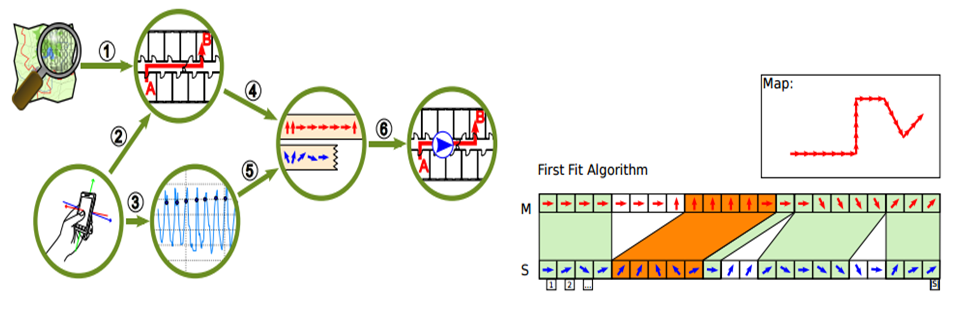
\includegraphics[width=.6\textwidth]{figures/acel.png}
\caption[Navegación mediante sensores inerciales \textit{First Fit} ]{\textbf{(a)} A la izquierda, proceso completo para la navegación utilizando acelerómetro y conteo de pasos. \textbf{(b)} A la derecha, método First-Fit para anticipar y predecir posición del usuario.\\
{\scriptsize (Fuente: \citep{6071934, 5766963})}}
\label{fig:acel}
\end{figure}

\textit{First Fit} realiza una especie de \textit{lookahead} para establecer el match con los pasos de la ruta y si los pasos que está detectando actualmente son errores. Con esto, puede mirar los pasos futuros y aproximar en donde se encuentra el usuario.

Los autores evalúan su propuesta en tres distintos escenarios, primero en exteriores para medir exactitud, luego en interiores para establecer si la solución es robusta, y luego en un escenario relativamente grande pero que es \textit{indoor}. Los autores concluyen que la solución es factible para la navegación, pero no para el posicionamiento, ya que es el usuario quien ingresa su posición estimada según ciertos nodos dentro del edificio. El sistema es escalable, pero requiere realizar las rutas predefinidas, lo cual puede ser mucho trabajo en edificaciones demasiado grandes.

\subsection{Comparativa de tecnologías \textit{Wireless}}

Dado que los mejores resultados presentes en la literatura corresponden a las tecnologías \textit{Wireless}, ya sean de sonido, radiofrecuencia, entre otros, a continuación, se muestran las ventajas y desventajas de cada una de ellas.

\begin{table}[!ht]
\centering
\caption[Comparativa Tecnologías Inalámbricas]{Tabla comparativa tecnologías inalámbricas}
\label{my-label}
\begin{tabular}{|c|c|c|c|c|c|}
\hline
            & Precisión {[}m{]}             & Rango {[}m{]} & Costo & Complejidad & Ambiente       \\ \hline
Infrarrojo  & \(10^{-2}\) - 1 & 1-5           & Alto  & Baja        & Indoor         \\ \hline
Ultrasonido & \(10^{-2}\)     & 2-10          & Medio & Baja        & Indoor         \\ \hline
Wi-Fi       & 1-10                          & 20-50         & Medio & Baja        & Indoor/Outdoor \\ \hline
RFID        & \(10^{-1}\)-1   & 1-10          & Bajo  & Baja        & Indoor         \\ \hline
Bluetooth   & 1-10                          & 1-30          & Bajo  & Baja        & Indoor/Outdoor \\ \hline
\end{tabular}
\end{table}

Ninguna tecnología presentada anteriormente es completamente efectiva en todos los escenarios, por lo que la elección de estas se debe hacer según las características del lugar, como su dinámica de cambio, obstáculos presentes, tamaño, entre otros. En la \autoref{fig:comparativa} se resume el alcance y características de cada tecnología de posicionamiento.


\begin{figure}[!ht]
\centering
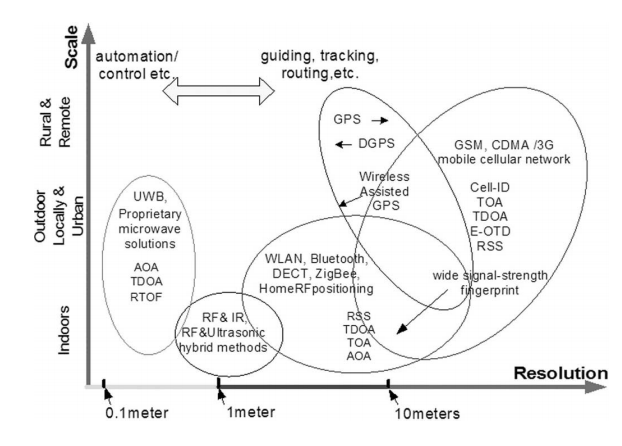
\includegraphics[width=.6\textwidth]{figures/comparativa.png}
\caption[Comparativa tecnologías inalámbricas]{Comparativa de distintas tecnologías inalámbricas basado en su resolución y alcance.\\
{\scriptsize (Fuente: \citep{Liu:2007:SWI:2220431.2221077})}}
\label{fig:comparativa}
\end{figure}


\section{Técnicas  matemáticas Wireless para localización indoor}

No es sencillo determinar un modelo completo para la propagación de ondas en interiores debido a muchos problemas que se presentan como lo es multipath, baja probabilidad de la línea de visión (LOS), y otros factores determinantes como tipo de material del edificio, superficies que reflejan ondas, el mismo cuerpo humano y objetos en movimiento. Por lo mismo es necesario establecer modelos matemáticos que reduzcan el error generado por la influencia de los factores antes mencionados.\\

Habitualmente se categorizan las técnicas matemáticas para la localización en interiores en 3 grandes grupos: Proximidad, Triangulación y \textit{fingerprint} (\textit{scene analysis}).

\subsection{Proximidad}

Es el método más simple, y se basa en determinar una posición simbólica y aproximada de la posición del usuario. Para lograrlo, existe una grilla de antenas o emisores de ondas de radio, y según la señal más fuerte detectada por el usuario, es donde se localiza en el sistema. Este tipo de localización es ampliamente usado en redes celulares, ya que permite determinar la posición de un dispositivo con una precisión de 50-200 m, sin embargo, no es buena en espacios reducidos. Por lo mismo se dice que este método tiene una alta varianza, y muchas veces no satisface la necesidad de localización. La ventaja es que al ser simple puede utilizarse en la mayoría de las redes inalámbricas, como lo es infrarrojo, RFID, Cell-ID, GSM.

Por lo anterior, habitualmente se dice que esta técnica es para saber en qué espacio geográfico o región está el usuario, no para saber su posición exacta \citep{Liu:2007:SWI:2220431.2221077}.

\subsection{Triangulación}

La triangulación utiliza las propiedades geométricas de un triángulo para estimar la posición del objeto.  La triangulación se divide en 2 puntos: lateración y angulación. Por una parte, la lateración estima la posición midiendo las distancias hacia múltiples puntos de referencia también llamados beacons. Angulación por su parte, no utiliza las distancias, sino que los ángulos relativos a cada beacon o punto de referencia. La  \autoref{fig:triangulacion} muestra cómo se calculan las posiciones relativas con lateración y angulación.

\begin{figure}[ht!]
\centering
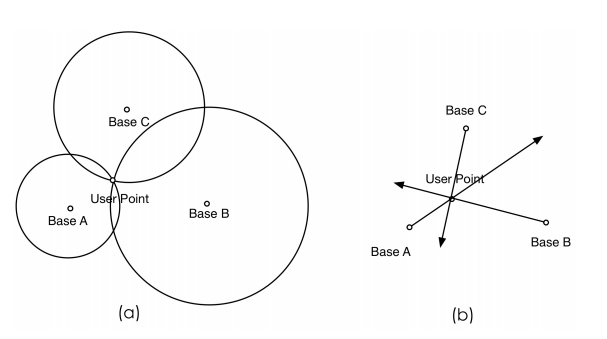
\includegraphics[width=.6\textwidth]{figures/triangulacion.png}
\caption[Lateración y Angulación]{Técnicas de triangulación basadas en lateración \textbf{(a)} y angulación \textbf{(b)}\\
{\scriptsize (Fuente: \citep{Liu:2007:SWI:2220431.2221077})}}
\label{fig:triangulacion}
\end{figure}

Si se conoce las \textit{base station} emisoras de ondas, lateración puede calcular la posición basado en un modelo matemático en donde se utiliza la intersección de tres círculos. Por otra parte, angulación utiliza la información del ángulo de llegada de las señales y con esto puede trazar 3 vectores, en donde la intersección representa la posición del objeto receptor.

El principal problema es establecer la distancia para lateración, y los ángulos para angulación. Para ello se han diseñado muchos acercamientos que permiten obtener esos valores.

\begin{enumerate}
\item \textbf{Técnicas de lateración }
\begin{enumerate}
\item \textbf{ToA (Time of arrival):} En ToA, la distancia del objeto móvil hacia las estaciones es directamente proporcional al tiempo de propagación, y además se sabe la velocidad de propagación de las ondas, que habitualmente es la velocidad de la luz siempre y cuando se transmitan en el aire. El dispositivo del usuario envía paquetes con las marcas temporales, es decir la hora en que se envía el paquete, luego la estación beacon puede determinar la hora en que llega el paquete, y haciendo la diferencia se obtiene el tiempo de propagación. ToA presenta dos grandes problemas, uno es que todos los dispositivos deben estar altamente sincronizados, y segundo, es que los paquetes deben estar etiquetados con información de tiempo de envió \citep{102710}.

\item \textbf{TDoA (Time difference of arrive):} Es similar a ToA, sin embargo en este caso no se necesita el tiempo de emisión del transmisor, solo se requiere el tiempo de llegada a cada uno de las estaciones base o beacons y mediante la diferencia de tiempo entre ellas establecer la posición. Para lograrlo, cada TDoA, se representa como una curva hiperbólica de las potenciales posiciones asumiendo distintos tiempos de transmisión como se muestra en la \autoref{fig:tdoa} . Donde se intersectan las curvas de a lo menos 2 estaciones beacons, es donde se transmitió la señal, por lo mismo es la posición del usuario.

\begin{figure}[ht!]
\centering
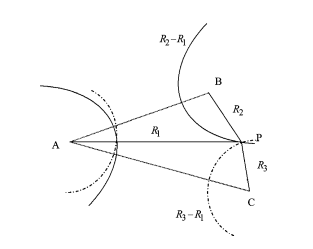
\includegraphics[width=.6\textwidth]{figures/tdoa.png}
\caption[Curvas Hiperbólicas TDoA]{Curvas hiperbólicas de TDoA que estiman la posición basado en el tiempo de transmisión.\\
{\scriptsize (Fuente: \citep{Liu:2007:SWI:2220431.2221077})}}
\label{fig:tdoa}
\end{figure}

Habitualmente por la complejidad del método, se utilizan linealización de las fórmulas del hiperboloide, a través de expansión en series de Taylor para luego crear algoritmos iterativos computacionalmente eficientes como se muestra en \citep{4103919}.

\item \textbf{Método basado en RSS (Received signal strength):}  Los métodos anteriores tienen algunos inconvenientes, primero, es complejo encontrar una línea de visión entre el emisor y receptor, además de la propagación por ondas de radio que puede presentar efectos de multicaminos, es decir, una misma onda llega al receptor por dos vías distintas, debido a la reflexión u otros factores. Una alternativa es estimar la distancia utilizando la atenuación de la fuerza la señal.

Existen modelos teóricos y empíricos, los cuales intentar predecir la distancia utilizando la diferencia entre la fuerza de la señal entre el transmisor y el receptor. Este método no es muy utilizado, debido al desvanecimiento de las señales en interiores, sin embargo puede utilizarse usando algunos pre procesamientos o mejoras, como por ejemplo establecer contornos predefinidos de señales RSS en forma de elipses como muestran los autores en \citep{1423549}.

\end{enumerate}

\item \textbf{Técnicas de angulación }
\begin{enumerate}
\item \textbf{AoA ( Angle of arrival):} Como se define en \citep{665} , la localización del objetivo puede realizarse mediante la intersección de múltiples líneas con una dirección dada por el ángulo entre cada estación y el receptor. Los métodos AoA deben utilizar al menos dos puntos de referencia o estaciones beacon,  y los dos ángulos respectivos con respecto al objeto que se quiere realizar la localización. La principal ventaja es que requiere tantas estaciones como el número de dimensiones en donde se requiere localizar el objeto, por ejemplo si se necesita determinar la posición en tres dimensiones, se requieren tres estaciones bases. Además, no se necesita sincronización de tiempos.

Por otra parte, es complejo y difícil de implementar, además de requerir software especializado, ya que para una localización muy precisa el ángulo debe ser medido con muy poco error y esto es difícil de lograr. Al igual que otras técnicas se ve afectado por propagación \textit{multipath} y desvanecimiento de las señales, interferencia y por la dirección de la apertura de medición. La \autoref{fig:angulacion} muestra el comportamiento de AoA.

\begin{figure}[ht!]
\centering
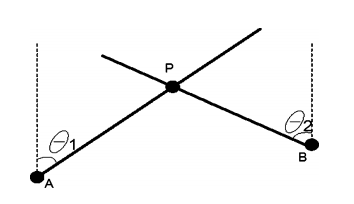
\includegraphics[width=.6\textwidth]{figures/angulacion.png}
\caption[Proyección de vectores AoA]{Proyección de vectores basado en ángulo de incidencia de las ondas sobre el objeto o dispositivo móvil.\\
{\scriptsize (Fuente: \citep{Liu:2007:SWI:2220431.2221077})}}
\label{fig:angulacion}
\end{figure}

\end{enumerate}
\end{enumerate}


\subsection{Fingerprint}

Se denomina \textit{fingerprint} o \textit{scene analysis} al tipo de algoritmos que en primer lugar recolecta características de un lugar y luego estima la localización en tiempo real utilizando las características, contrastándolas con las características actuales. Lo más habitual es utilizar Fingerprint basado en RSS.

Fingerprint presenta dos etapas, la etapa offline y la etapa online. Durante la etapa offline se realiza un reconocimiento de las características del lugar, en donde se mide las coordenadas de cada estación base y la fuerza de la señal en determinados lugares, obteniendo así un mapa de señales del entorno.  Durante la etapa online se utiliza la señal actual recibida de cada estación base y un modelo generado en la etapa offline, generando así una estimación de la posición del usuario. La  \autoref{fig:finger} muestra el funcionamiento a nivel general de Fingerprint:

\begin{figure}[ht!]
\centering
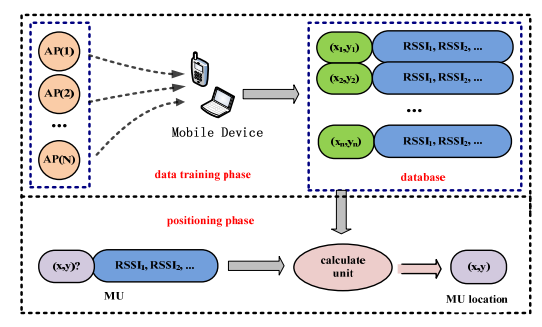
\includegraphics[width=.6\textwidth]{figures/finger.png}
\caption[Proceso de creación Fingerprint]{Proceso de captura de características Fingerprint y elaboración del modelo para estimar la posición.\\
{\scriptsize (Fuente: \citep{Liu:2007:SWI:2220431.2221077})}}
\label{fig:finger}
\end{figure}

Fingerprint se divide en dos grandes aristas, \textit{map-based Fingerprint} y \textit{map-free} Fingerprint:

\begin{enumerate}
\item \textbf{Map-based Fingerprint}

Este caso utiliza la etapa offline y online, en donde en la etapa offline se generan los radio-map de cada posición, es decir, asociar una característica de las señales según la posición geográfica en donde se toma la medición. Existen dos tipos de radio-map, los cuales son radio-map de tipo valor medio, y radio-map de tipo función de densidad de probabilidad. En el radio-map de tipo valor medio existe un número limitado de puntos en donde se toman las mediciones de las señales, mientras que el radio-map de tipo función de densidad de probabilidad, puede representar todos los puntos del lugar como una función continua. Para la estimación de la posición se han realizado variados acercamientos como es modelos de probabilidad, kNN, redes neuronales, SVM, estimación de máxima verosimilitud, estimación bayesiana \citep{Liu:2007:SWI:2220431.2221077, 1192765}.

Para la generación de los radio-maps se utiliza habitualmente tres técnicas, las cuales son \textit{Model Based Estimation}, Medición Offline y calibración Online. \textit{Model Based Estimation} no confía plenamente en las señales RSS, si no que utiliza distintos modelos de propagación como son \textit{Wall attenuation factor} \citep{Bahl00radar:an} , 2D-ray tracing y otros modelos de propagación de las señales para estimar la fuerza de la señal en determinados puntos del espacio y generar el radio-map. La siguiente ecuación describe la fórmula de la atenuación de señales por el efecto de las paredes.

\begin{equation}
P(d)[dBm] = P(d_{0})[dBm] - 10nlog (\frac{d}{d_{0}}) - \left\{ \begin{array}{lcc}
             nW*WAF &   si  & nW < C \\
             \\ C*WAF &  si & nW \geq C \\
             \end{array} \right.
\end{equation}

   

En donde \(n\) representa la velocidad con la que aumenta la pérdida de poder de la señal con la distancia. \(P(d_{0})\) es el poder de la señal en cierto punto de referencia \(d_{0}\) y \(d\) es la distancia que separa al transmisor y receptor. \(C\) es el máximo número de paredes para el cual el factor de atenuación hace alguna diferencia. \(nW\) es el número de paredes y \(WAF\) es el factor de atenuación por las paredes. Habitualmente \(n\) y \(WAF\) se conocen, ya que depende del lugar y orden de los objetos dentro de un edificio.

Por otra parte, se tiene mediciones offline, en donde se realiza un proceso lento y tedioso, de medir cada punto del lugar en donde se realiza la localización. Mientras más puntos se registran, mejor será el radio-map ya que tiene un mayor número de datos de entrenamiento. Para reducir el trabajo, algunos autores han utilizado robots para registrar la medición de las señales \citep{5398451}. La Figura \autoref{fig:robots} muestra cómo se utiliza un robot para tomar mediciones de las señales en determinados puntos, en este caso los beacons corresponden a tags RFID.

\begin{figure}[ht!]
\centering
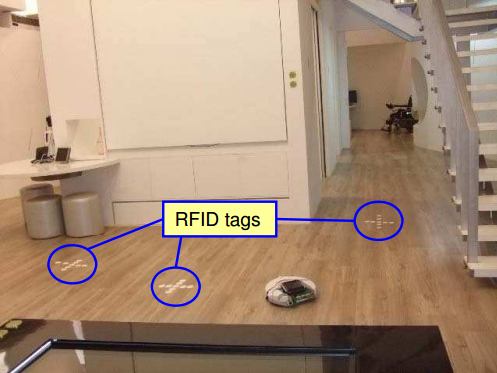
\includegraphics[width=.4\textwidth]{figures/robots.png}
\caption[Robots para map Fingerprint]{Robot que toma automáticamente las características para elaborar el mapeo fingerprint de un determinado lugar.\\
{\scriptsize (Fuente: \citep{Liu:2007:SWI:2220431.2221077})}}
\label{fig:robots}
\end{figure}

Por último, calibración online tiene en cuenta que se requiere mucho esfuerzo para realizar las mediciones y obtener las características de señales, además si el entorno cambia constantemente es probable que las señales también cambien y todo el registro se pierda y deba ser realizado nuevamente. Entonces calibración online combina las dos técnicas anteriores, dejando ciertos nodos ancla que miden constantemente la señal en esos puntos, y mediante \textit{model based estimation}, pueden estimar la fuerza de la señal en otros lugares en donde no hay nodos ancla. Los nodos ancla pueden realizar mediciones cada cualquier intervalo de tiempo, ajustando el modelo, y por lo mismo no se ve afectado por cambios en el entorno.

\item \textbf{Map-Free Fingerprint} 

Map-based fingerprint puede utilizarse con cualquier red inalámbrica o incluso otros tipos de Fingerprint, como ultrasonido, campos magnéticos, entre otros. Sin embargo la complejidad para registrar mediciones aumenta cuando el área a mapear aumenta, además la mantención temporal del radio-map es un proceso engorroso y lento. Map-free reduce esta complejidad, utilizando otras formas de localizar usando fingerprints.

En \cite{Wang:2012:NNW:2307636.2307655} el autor observa patrones de las señales en ciertos lugares como el ascensor o el pasillo, y con estos puntos de referencia utiliza aprendizaje no supervisado para estimar la posición del usuario. Combinando esta información junto con los acelerómetros y sensores del dispositivo móvil, el autor muestra cómo puede obtener una posición estimada muy cercana a la real. Entonces este tipo de Fingerprint, se basa en el patrón del punto de referencia actual y las mediciones de puntos de referencia anteriores. Por lo mismo se dice que este método no soporta localización estática.

\end{enumerate}

\subsubsection{Formulación del problema Fingerprint}

En la técnica de \textit{Fingerprint} el área es dividida en un conjunto de puntos de referencia (RPs), \(P = \{p_{j} = (x_{j}, y_{j}) \ | \ j = 1,...,N\}\) en donde \(P\) define el conjunto cartesiano de RPs, que no necesariamente son un conjunto de puntos equidistantes entre si \citep{7874080}. El dispositivo móvil graba un conjunto de mediciones \textit{Fingerprint} RSS en los instantes \(t_{m} ,\ m = 1,...,M\) con magnitudes RSS \( \ r_{j}^{i}(t_{1}),..., r_{j}^{i}(t_{M}) \ \) en cada RP, donde \(i\) indica el índice del access point desde el conjunto de access points \( \mathcal{L} = \quad \{AP^{1}, ..., AP^{L}\}\). Generalmente se toma el mismo número de ejemplos de entrenamiento, \(M\) en cada RP. Los Fingerprints RSS de todos los access point en el tiempo \(t_{m}\) en el punto \(p_{j}\) están organizados en un vector \(r_{j}(t_{m}) = [(r_{j}^{1}(t_{m}),...,(r_{j}^{L}(t_{m})]^{T}\). El radio map completo guardado en el instante \(t_m\) puede ser reconocido por la siguiente matriz:


\begin{align}
\def\arraystretch{2.2}
   R(t_{m}) = (\textbf{r}_{1}(t_{m}), ..., \textbf{r}_{N}(t_{m})) = 
  \left[ {\begin{array}{cccc}
   r_{1}^{1}(t_{m}) & r_{2}^{1}(t_{m}) & ... & r_{N}^{1}(t_{m}) \\
   r_{1}^{2}(t_{m}) & r_{2}^{2}(t_{m}) & ... & r_{N}^{2}(t_{m}) \\
   r_{1}^{3}(t_{m}) & r_{2}^{3}(t_{m}) & ... & r_{N}^{3}(t_{m}) \\
   r_{1}^{4}(t_{m}) & r_{2}^{4}(t_{m}) & ... & r_{N}^{4}(t_{m}) \\
  \end{array} } \right] \ , \quad 
m\ = \ 1,...,M.
\end{align}
 

Un subconjunto de RPs con el mayor grado de similaridad es denotado como \(\mathcal{K}\) y está definido como \(\mathcal{|K|} = K\). Esta similaridad es definida por cada método y es detallada posteriormente.

En la fase online el usuario recibe una medición RSS \quad \(\textbf{y} = (y^{1}, ..., y^{M}) ^{T}\). Entonces el objetivo es simple; encontrar la localización \(\hat{\textbf{p}} = ( \hat{x}, \hat{y})\), basado en una regla que compara la medición online contra el radio map de \textit{fingerprints} como: 

\begin{equation}
\hat{\textbf{p}} = f(\textbf{R}, \textbf{y})
\end{equation}

En donde \(R\) denota la colección de radiomaps en todas las instancias guardadas. A continuación, se muestran los tres acercamientos principales para la localización utilizando Fingerprint.

\subsubsection{Acercamientos convencionales de Fingerprint}

\begin{enumerate}
\item \textbf{Acercamiento determinista:} En esta forma de resolver el problema de Fingerprint, la posición que logra la mayor similaridad con la posición real es alcanzada utilizando la siguiente formulación:

\begin{equation}
\hat{\textbf{p}} = \underset{j=1,...,N}{\mathrm{argmin}} \quad d( \breve{\textbf{r}}_{j}, \textbf{y})
\end{equation}

En donde \(\breve{\textbf{r}}\) es el valor representativo del Fingerprint en el \(j-esimo\) RP \citep{832252} y \(d( \breve{\textbf{r}}_{j}, \textbf{y}) \) define una medida de distancia típica \citep{6817920}. En el caso de promedio de tiempo, el valor representativo es el promedio de los Fingerprints durante el tiempo en que fueron medidos. La distancia Euclidiana también puede ser utilizada, definida como: 

\begin{equation}
d( \breve{\textbf{r}}_{j}, \textbf{y}) = \lVert y - \breve{\textbf{r}}_{j} \rVert_{2} \quad j = 1,..., N.
\end{equation}
   

Ya que el número de access point disponibles  varia en la superficie a localizar, la posición es típicamente estimada sobre los AP visibles y los AP desconocidos se estiman en un valor que indica una señal débil o un valor imposible de obtener (100 dBm).

\item \textbf{Acercamiento probabilista:} En este acercamiento, una sola medida RSS puede ser no suficiente para estimar la posición, ya que no representa la variación temporal de los datos en la propagación en interiores. El desempeño del acercamiento determinista puede ser mejorado si en vez de utilizar solo un subconjunto de Fingerprints RSS, todos los Fingerprints son utilizados. En esta presunción se basa el acercamiento estadístico, utilizar todos los Fingerprints para describir de mejor manera el área en cuestión.

La forma en que el acercamiento estadístico estima la posición, se basa en la estimación de Máximo a Posteriori ( MAP) \citep{4907834}, de esta manera MAP estima la posición del usuario maximizando la probabilidad condicional de la posición dado la medición recibida en la etapa online:

\begin{equation}
\hat{\textbf{p}} = \underset{j=1,...,N}{\mathrm{argmax}} \quad f( \textbf{p}_{j} \vert \textbf{y})
\end{equation}

 En donde \( f( \textbf{p}_{j} \vert \textbf{y}) \) es la probabilidad condicional de que el usuario este en \(\textbf{p}_{j}\) dado que recibió el vector \( y \) en la etapa online.
 
Gracias al teorema de Bayes esto puede ser re formulado de la siguiente manera:

\begin{equation} \label{eq:1}
 f( \textbf{p}_{j} \vert \textbf{y}) = \frac{f( \textbf{p}_{j} , \textbf{y})}{f(y)} = \frac{f( \textbf{y} \vert \textbf{p}_{j}) f(\textbf{p}_{j})} {\sum_{j=1}^{N} f( \textbf{y} \vert \textbf{p}_{j}) f(\textbf{p}_{j})} \quad j = 1, ..., N 
\end{equation}

La probabilidad \(f(\textbf{p}_{j})\) es la distribución de la posición del usuario sobre el área completa, y se asume generalmente uniforme ya que no existe conocimiento previo en la posición del usuario, por lo que todos los puntos estudiados son equiprobables. Por lo anterior, \(f(\textbf{p}_{j})\) puede ser ignorado en el problema de maximización, de esta forma el denominador en la ecuación \ref{eq:1} es el mismo para todo \( j= 1, ..., N\) de esta manera, el problema MAP es transformado a :

\begin{equation}
\hat{\textbf{p}} = \underset{j=1,...,N}{\mathrm{argmax}} \quad f( \textbf{y}  \vert \textbf{p}_{j})
\end{equation}


Conocido comúnmente como el estimador de máxima verosimilitud o \textit{Maximum Likelihood (ML)}. 

Lo anterior revela que el acercamiento determinista confía en estimar la densidad a priori \(f( \textbf{y} \ \vert \ \textbf{p}_{j})\). Existen dos formas utilizadas en la estimación de esta distribución de densidad de probabilidad, las cuales son denominadas paramétrica y no paramétrica. La estimación paramétrica trata a la distribución de probabilidad como una distribución analítica conocida, por ejemplo una distribución Gaussiana \citep{Haeberlen:2004:PRL:1023720.1023728} para aproximar las características temporales de las señales RSS. Este enfoque ha sido cuestionado en múltiples investigaciones, debido a lo poco realista que se torna este supuesto en muchos lugares y recintos experimentales. Los primeros acercamientos utilizaban una aproximación log-normal para la distribución, sin embargo, es sesgada y estacionaria sobre pequeños intervalos de tiempo.  Las aproximaciones modernas de estimación paramétrica utilizan funciones Kernel para lograr mejores resultados. 

La estimación no paramétrica no asume nada con respecto a la distribución de Fingerprint RSS. En vez de esto, la distribución es generada utilizando un histograma que cuadra con el radio map construido \citep{Haeberlen:2004:PRL:1023720.1023728, Ladd:2002:RLS:570645.570674}. En este emparejamiento, todos los datos son cuantizados en múltiples niveles y la frecuencia de cada barra del histograma es calculada, para la estimación de \(f( \textbf{y} \ \vert \ \textbf{p}_{j} ) \). El histograma consiste entonces en la concatenación de todas estas barras. Sin embargo, un gran número de ejemplos son necesarios en diferentes instantes de tiempo en cada RP para generar el histograma, lo que es complejo de obtener en la práctica.

\item \textbf{Técnicas de reconocimiento de patrones:} La idea básica de reconocimiento de patrones se basa en clasificadores, que son utilizados con los Fingerprints recolectados y luego son capaces de discriminar una nueva medición RSS desconocida durante la fase online. En la fase de entrenamiento de cada clasificador, el sistema ajusta los parámetros del modelo, mediante el uso del radio map de Fingerprints recolectados en forma de base de datos. En la fase de testing, los datos RSS recibidos desde una posición desconocida son analizados por el clasificador para estimar la posición más cercana. La diferencia entre los algoritmos de reconocimiento de patrones, son en la manera en que utilizan técnicas para emparejar los datos. La salida de estos algoritmos es generalmente un conjunto de probabilidades o verosimilitud de muchas posiciones, con lo cual es posible estimar un centroide de todas las posiciones como solución, o simplemente elegir el que posea la mayor probabilidad.
\end{enumerate}

\subsubsection{Avances recientes en Fingerprint}

La presente sección pretende mostrar los últimos avances en las técnicas de Fingerprint con el objetivo de esclarecer las ventajas y desventajas de estos. Antes se presenta un diagrama de cómo funciona Fingerprint en su forma general:

\begin{figure}[ht!]
\centering
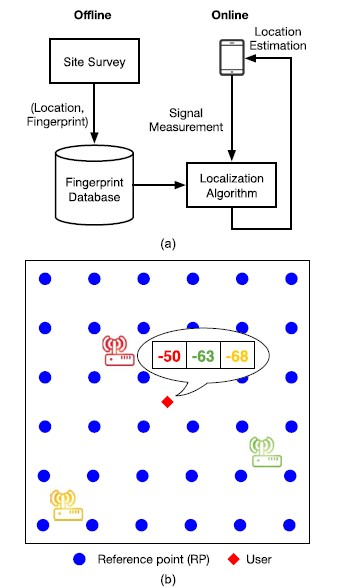
\includegraphics[width=.4\textwidth]{figures/fingerprint_basic.jpg}
\caption[Fingerprint esquema básico]{(a) Flujo básico de fingerprint. (b) radio-map de un sistema de localización indoor\\
{\scriptsize (Fuente: \citep{7174948})}}
\label{fig:fingerprint_basic}
\end{figure}

\begin{enumerate}
\item \textbf{Explotando patrones temporales y espaciales:} El Fingerprint tradicional se basa en la medición de vectores RSS. Debido al ruido en las mediciones, el objetivo puede ser \textit{mapeado} a una posición distinta de vectores de señales similares \citep{6681592}. La precisión puede ser aumentada si son considerados patrones espaciales y temporales, característicos del lugar en el cual se está experimentando.

\begin{itemize}
\item \textbf{Patrones temporales} Son patrones de señales que son encontrados a medida que se camina por el área en donde se desea posicionar. Estos patrones pueden ayudar a mejorar la localización en interiores. Luego, cuando un vector de señales es comparado en una posición fija, los patrones contienen información temporal que pueden ser utilizados para restringir y corregir las señales RSS para la localización base.

\item \textbf{Patrones espaciales} Están caracterizados por asociar señales RSSI con su correspondiente distribución geográfica. Mientras que los patrones temporales requieren conocer el movimiento del usuario, el cual puede ser no determinado o poco preciso en casos reales. Los patrones geográficos de señales pueden ser utilizados para restringir la posición del usuario. Estos patrones incluyen orden de los vectores RRSI, puntos de control en las señales, y la cobertura de las señales dadas por los APs.

\end{itemize}

\item \textbf{Localización colaborativa entre móviles} Muchos de los avances se enfocan principalmente en determinar la posición de un usuario independientemente de los demás dispositivos, sin considerar sus posiciones relativas. Debido a los errores de cada móvil independiente, dos objetivos físicos cercanos pueden ser marcados en diferentes posiciones estimadas. Entonces, si la información de la posición relativa puede ser accedida y utilizada, los resultados en la estimación pueden ser mejorados para la localización individual de cada móvil. Trabajos recientes han desarrollado la localización colaborativa. Estas aristas nacen básicamente de las siguientes tendencias en computación móvil:

\begin{itemize}
\item \textbf{Contexto de localización de interacción social:} En la localización indoor, la gente puede estar cercana en escenarios sociales típicos \citep{Chan2006}. En museos, por ejemplo, la gente busca dentro junto a su familia o amigos. La interacción entre este conjunto determina un patrón de localización.

\item \textbf{Dispositivos móviles penetrantes y sensores avanzados:} En estos días, los \textit{smartphones} han desarrollado muchos sensores, los cuales pueden detectar otros móviles en su vecindario cercano, basado en uno o varios protocolos, como puede ser Bluetooth, WiFi direct, NFC y ondas de sonido. El aumento de los dispositivos móviles con estos sensores provee la posibilidad de mejorar significativamente esta técnica en posteriores investigaciones.
\end{itemize}


\item \textbf{Localización asistida por movimiento: } La localización asistida por movimiento es una de las técnicas híbridas más utilizadas en estos días, debido a la gran penetración en el mercado de dispositivos que presentan sensores en el ámbito móvil. Los más grandes avances consisten en las siguientes dos técnicas:

\begin{itemize}
\item \textbf{Avances en la medición de movimiento:} El monitoreo del comportamiento de una caminata es importante para la localización asistida en movimiento precisa. El mayor desafió en obtener información del movimiento es que los sensores inerciales de los dispositivos móviles sufren de calibración imperfecta y mediciones con ruido. \textit{Step counting} es el mayor acercamiento para capturar el movimiento y dirección de una caminata \citep{6407455}. Trabajos recientes apuntan a mejorar la dirección de la caminata, conteo de pasos y longitud de pasos. Sin embargo, como adaptar estos parámetros a cada usuario, es decir, sus propios perfiles de movimiento es un área desafiante que continua en investigación.

\item \textbf{Modelos de fusión avanzados y eficientes:} Como fusionar el movimiento con y la detección de señales RSS es esencial para mejorar la precisión en la localización en interiores. El modelo usado en fusión necesita capturar la correlación (ya sea temporal o espacial) entre las señales medidas. Sin embargo, si el modelo es altamente complejo, el alto costo computacional también afecta la calidad de la estimación en la localización. A pesar de esto, buscar un algoritmo de fusión eficiente y preciso se ha convertido recientemente en una importante tendencia para la localización asistida por movimiento \citep{6846747}.

\end{itemize}
\end{enumerate}
